\begin{figure}
  \begin{subfigure}{0.24\linewidth}
    \centering
    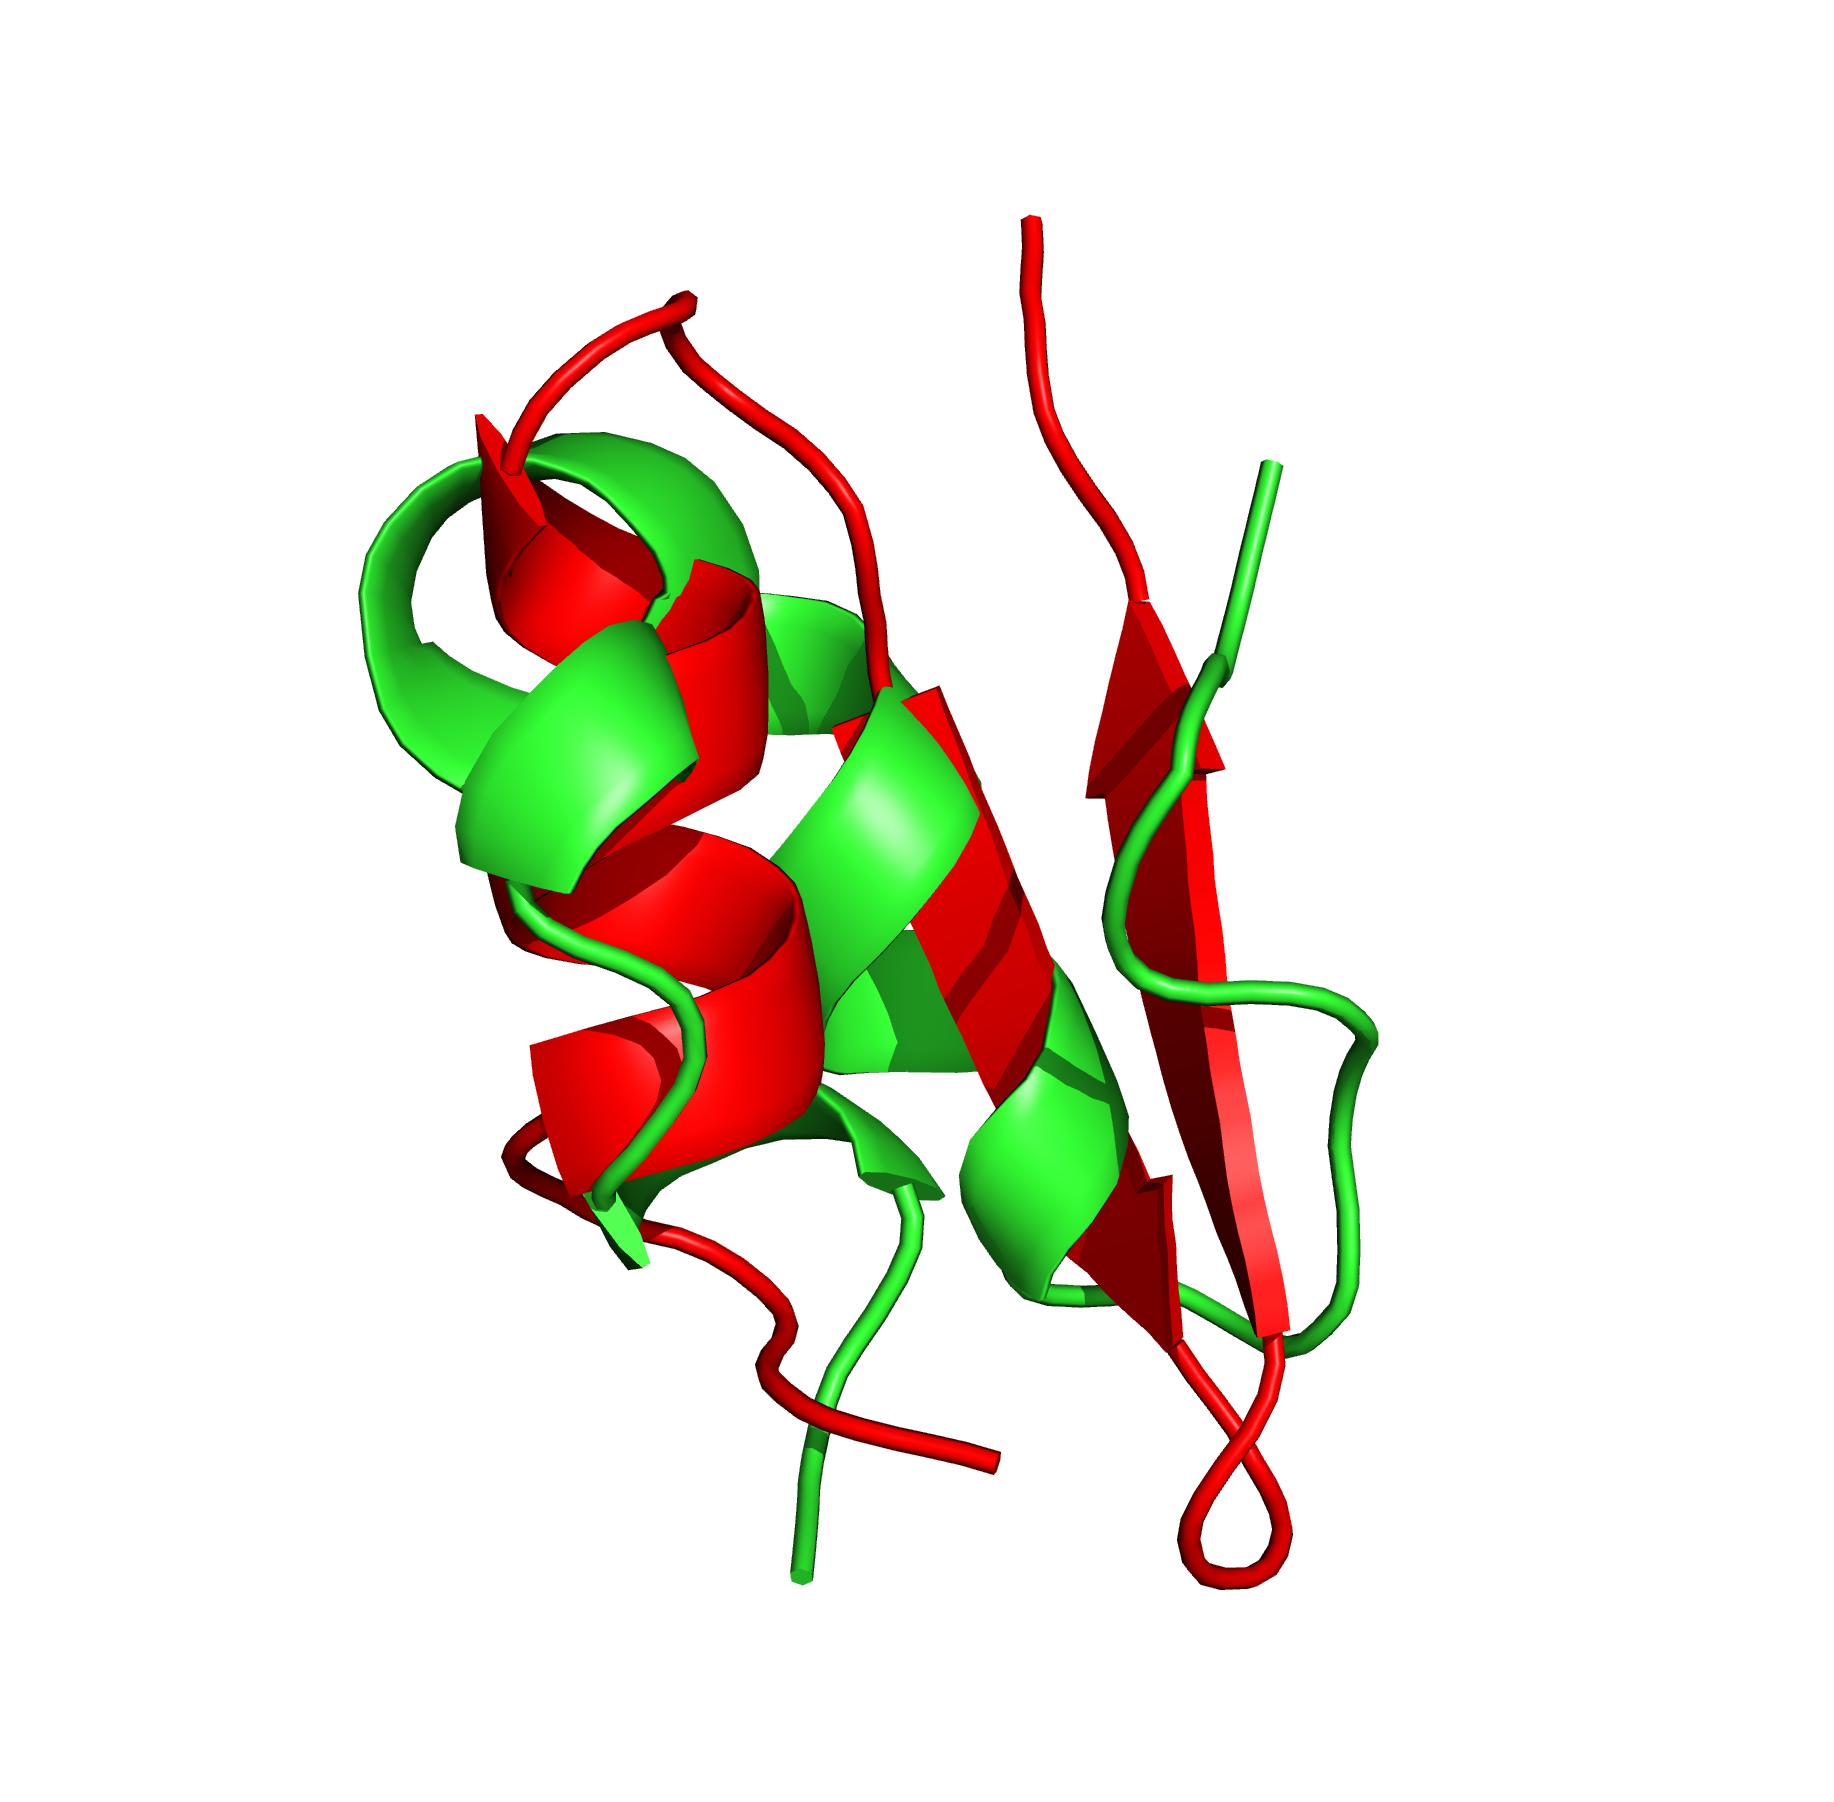
\includegraphics[width=0.9\linewidth]{Figuras/prots/1acw_render.png}
    \caption{1acw (4.45\AA)}
    \label{fig:1acw-conformation}
  \end{subfigure}
%
  \begin{subfigure}{0.24\linewidth}
    \centering
    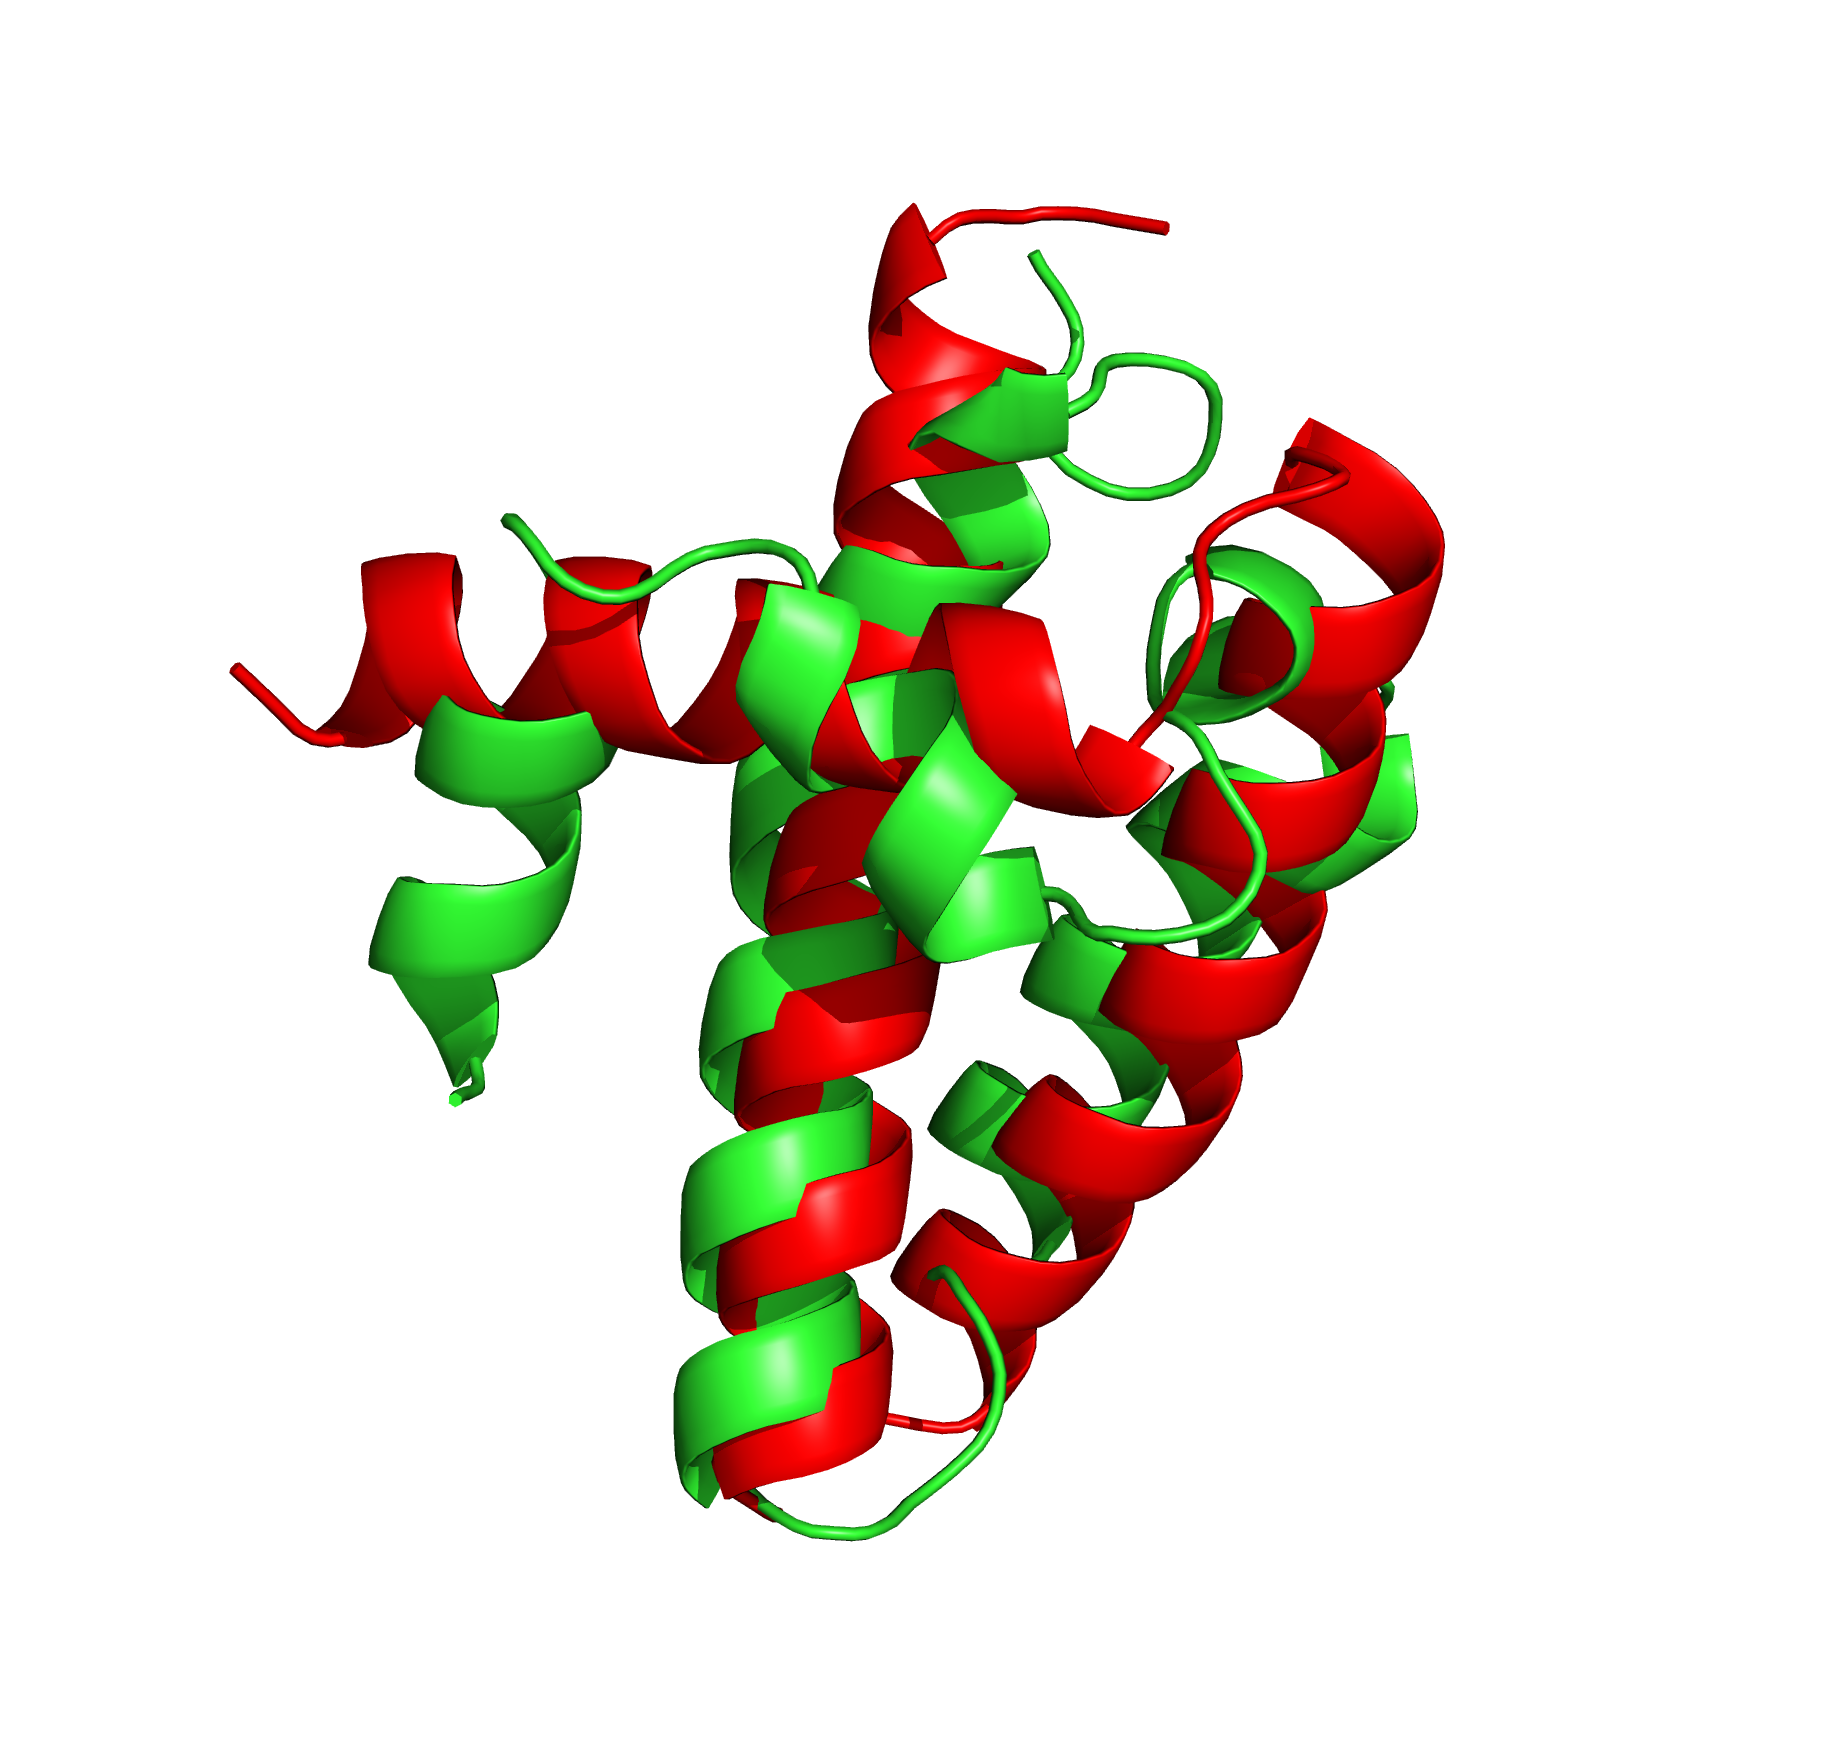
\includegraphics[width=0.9\linewidth]{Figuras/prots/1ail_render.png}
    \caption{1ail (4.26\AA)}
    \label{fig:1ail-conformation}
  \end{subfigure}
%
  \begin{subfigure}{0.24\linewidth}
    \centering
    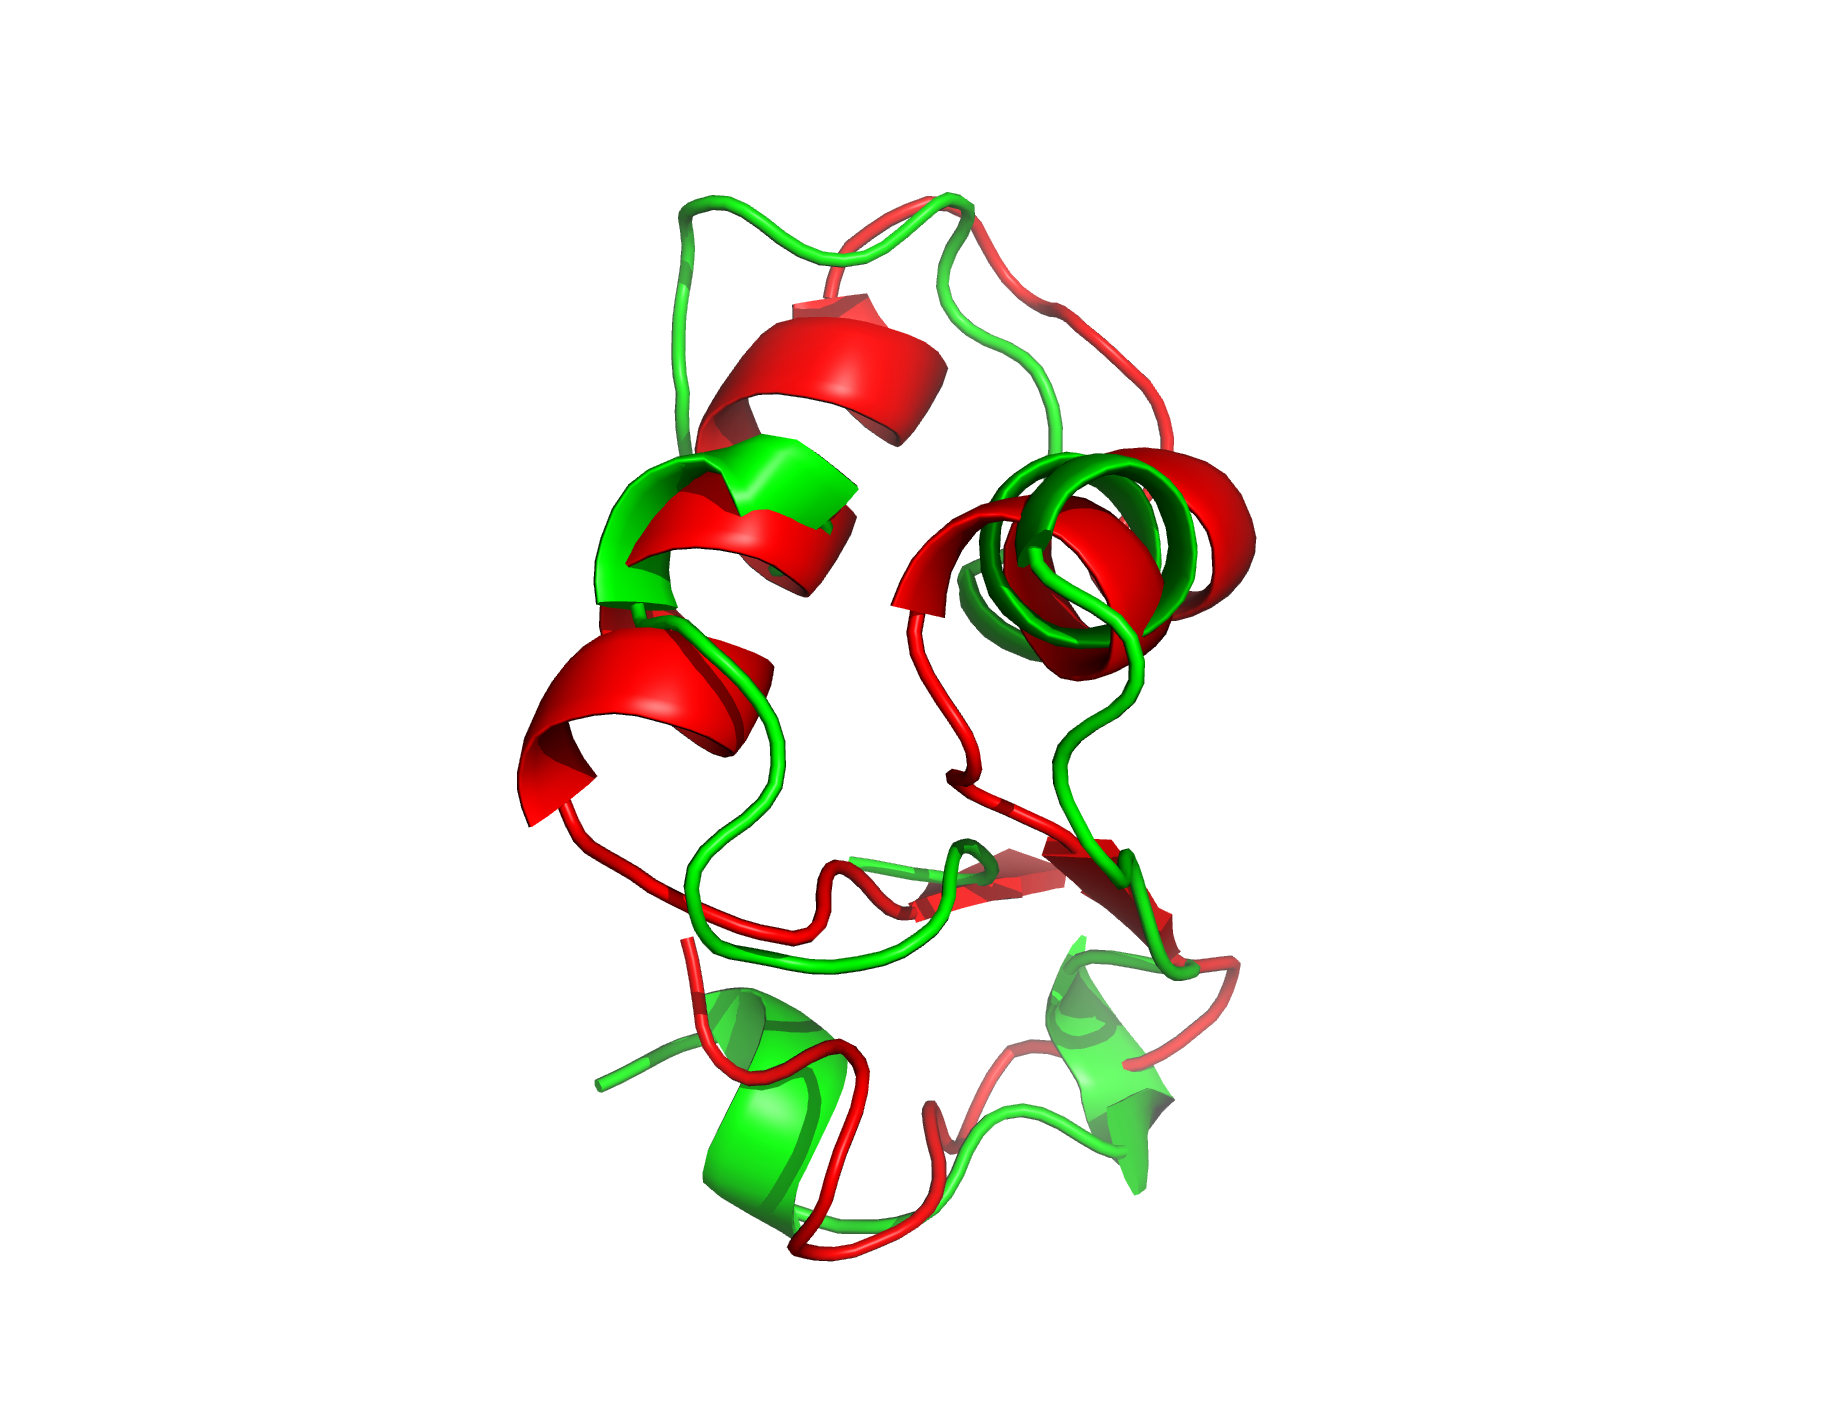
\includegraphics[width=0.9\linewidth]{Figuras/prots/1crn_render.png}
    \caption{1crn (4.18\AA)}
    \label{fig:1crn-conformation}
  \end{subfigure}
%
  \begin{subfigure}{0.24\linewidth}
    \centering
    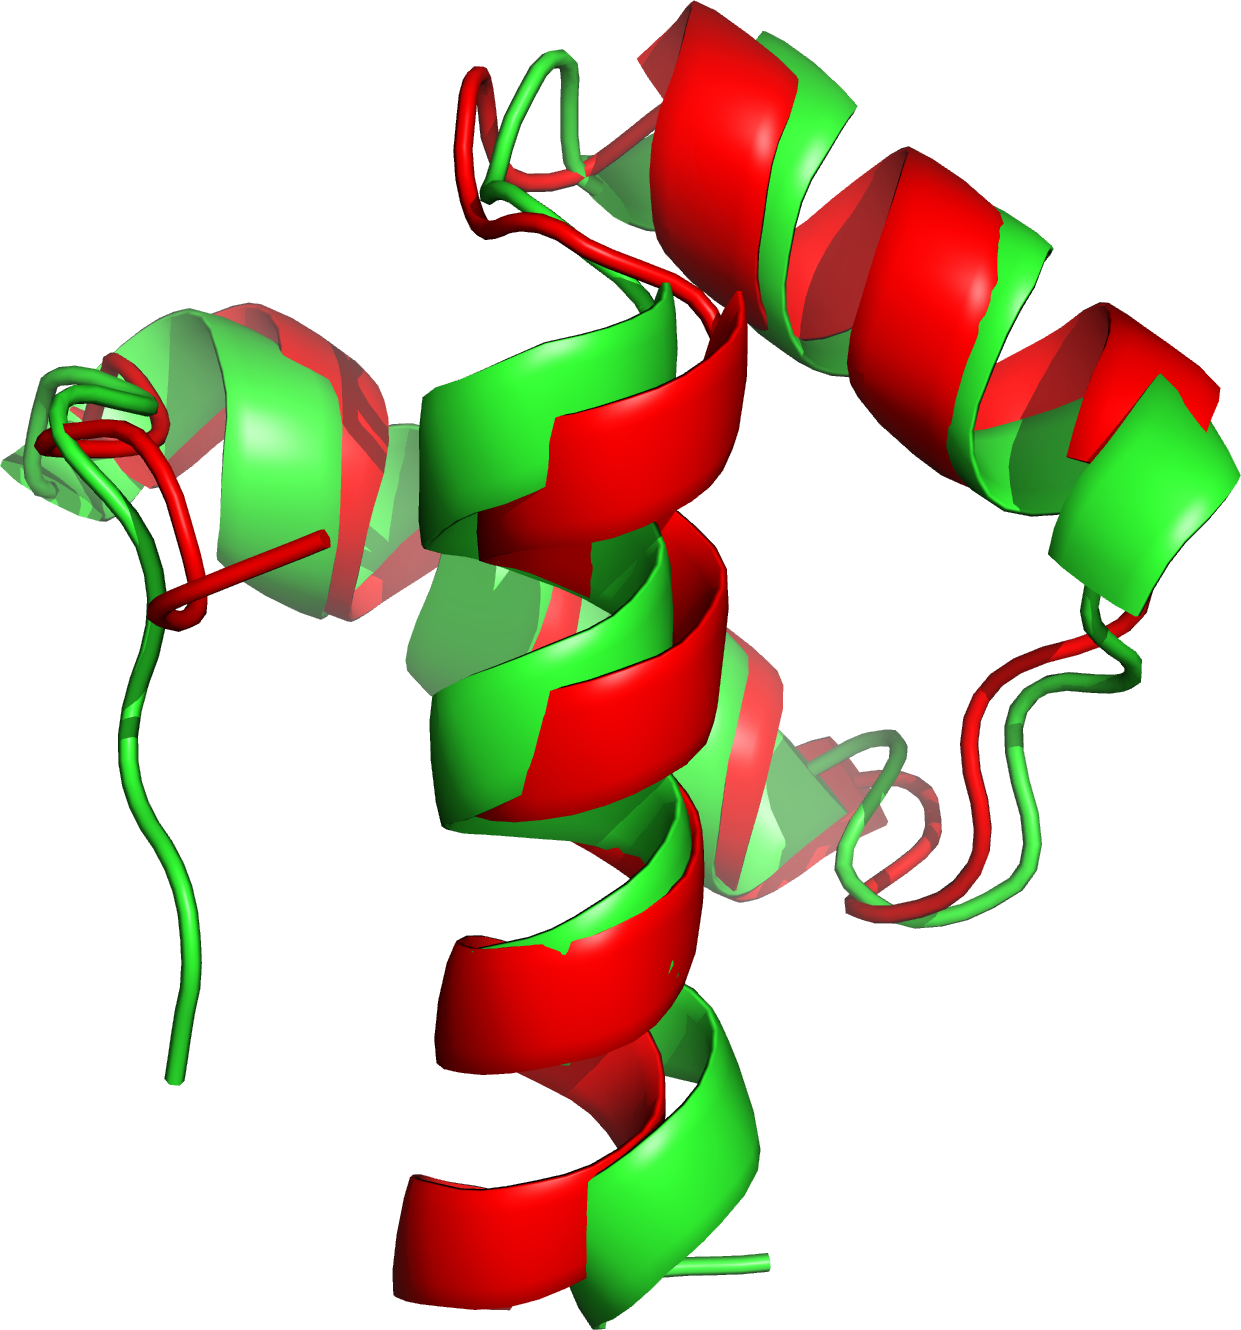
\includegraphics[width=0.9\linewidth]{Figuras/prots/1enh_render.png}
    \caption{1enh (2.65(\AA))}
    \label{fig:1enh-conformation}
  \end{subfigure}
% \end{figure}
% \begin{figure}
  \begin{subfigure}{0.32\linewidth}
    \centering
    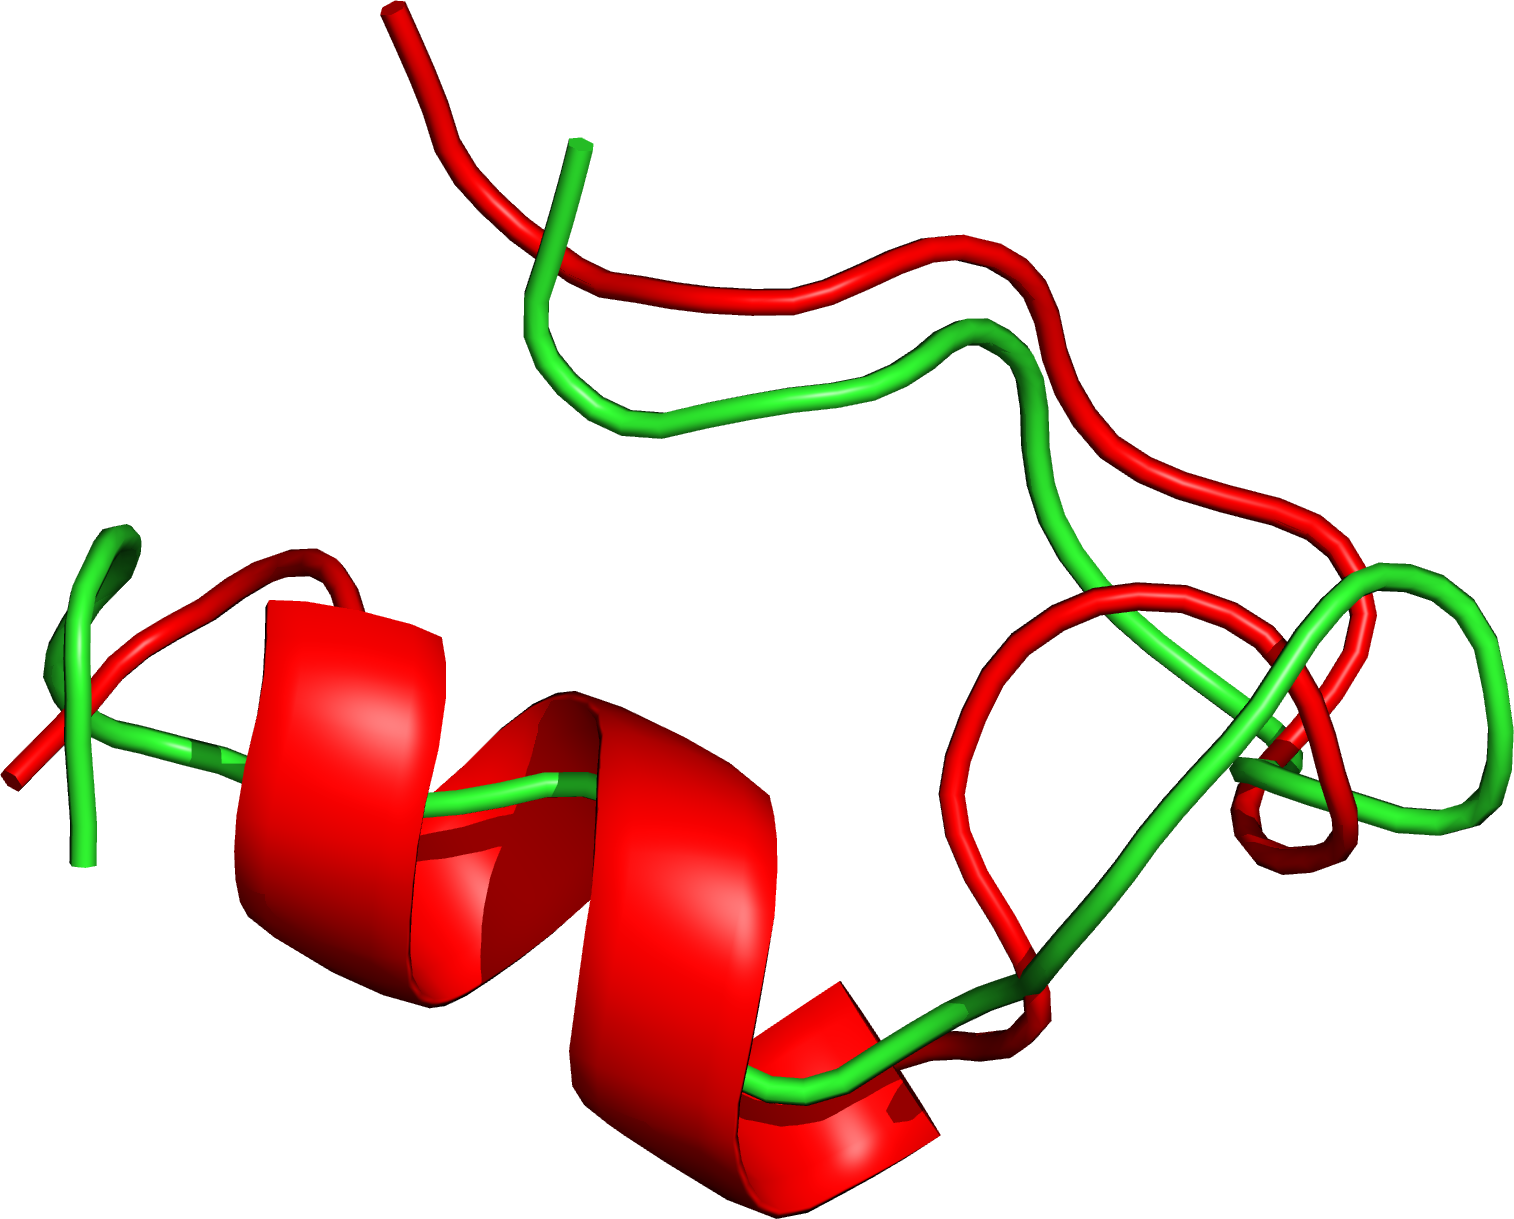
\includegraphics[width=0.9\linewidth]{Figuras/prots/1l2y_render.png}
    \caption{1l2y (3.39\AA)}
    \label{fig:1l2y-conformation}
  \end{subfigure}
%
  \begin{subfigure}{0.32\linewidth}
    \centering
    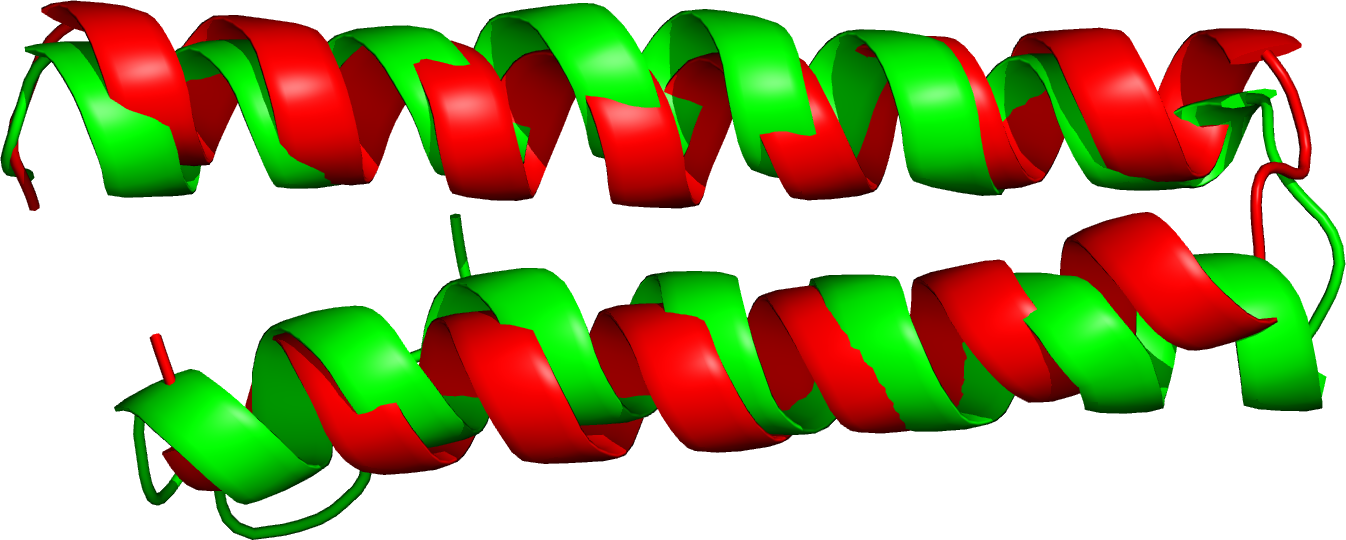
\includegraphics[width=0.9\linewidth]{Figuras/prots/1rop_render.png}
    \caption{1rop (2.18\AA)}
    \label{fig:1rop-conformation}
  \end{subfigure}
%
  \begin{subfigure}{0.32\linewidth}
    \centering
    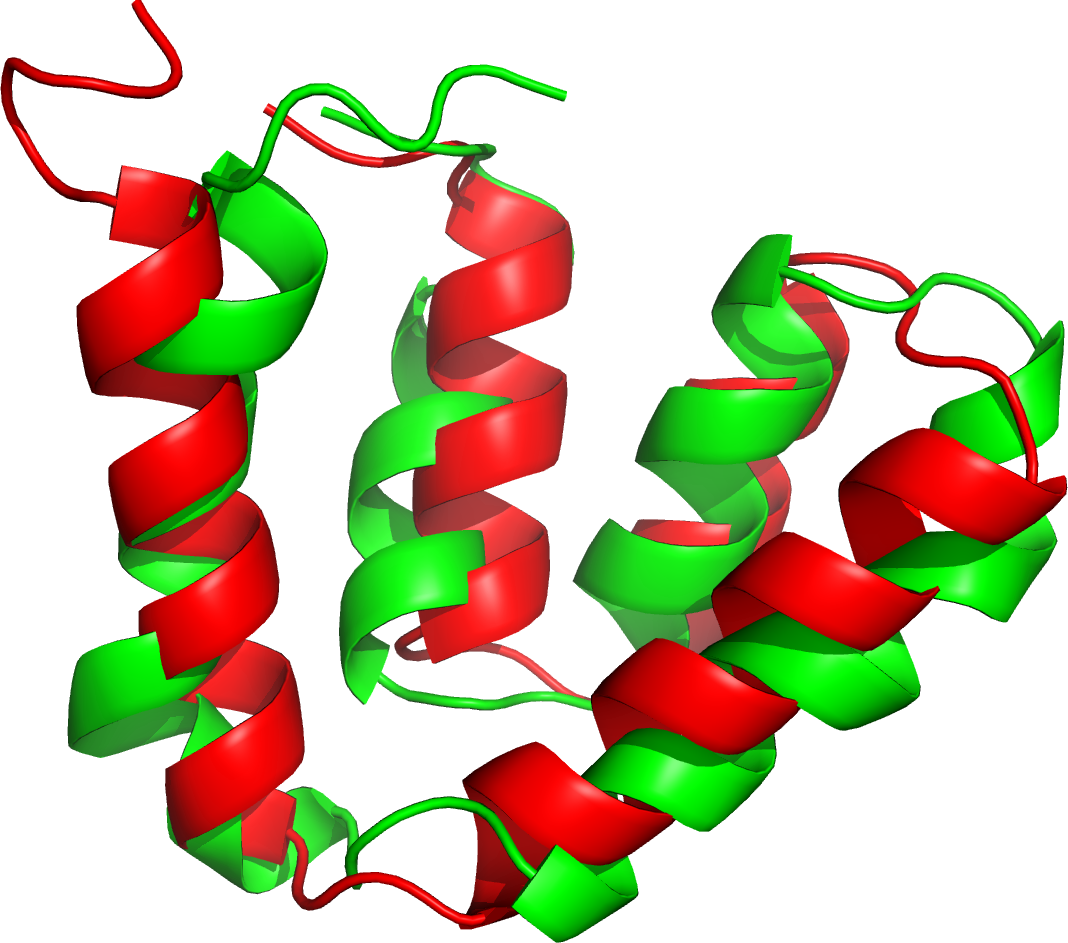
\includegraphics[width=0.9\linewidth]{Figuras/prots/1utg_render.png}
    \caption{1utg (4.41\AA)}
    \label{fig:1utg-conformation}
  \end{subfigure}
% \end{figure}
% \begin{figure}
  \begin{subfigure}{0.32\linewidth}
    \centering
    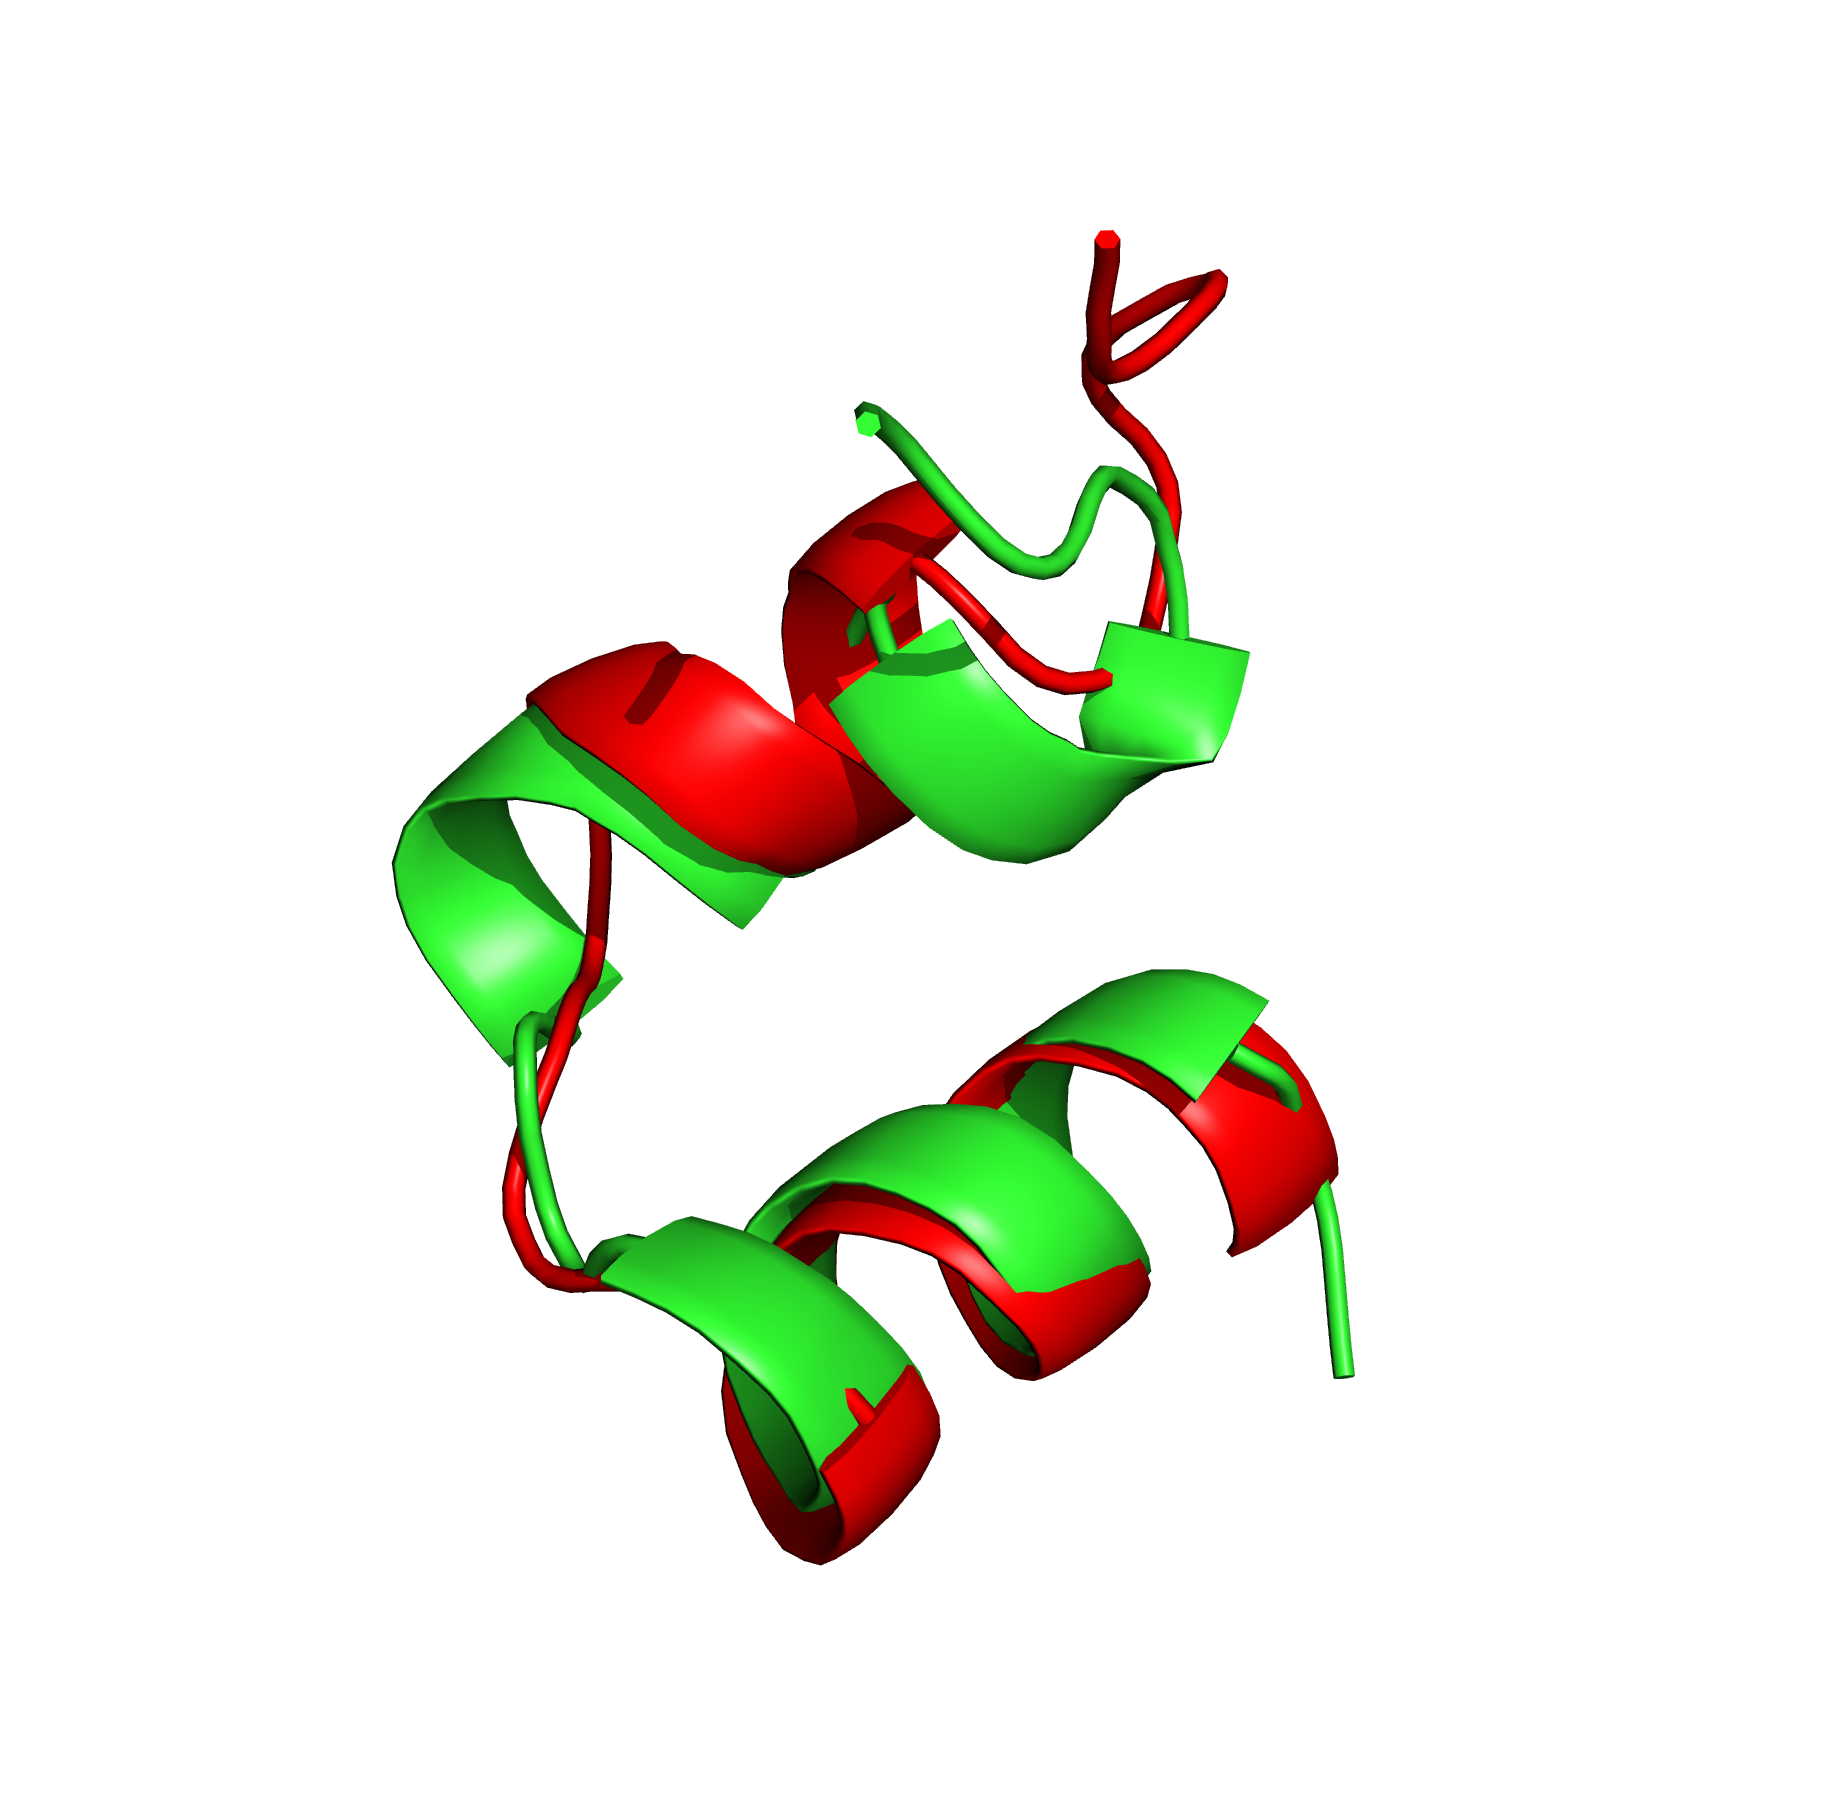
\includegraphics[width=0.9\linewidth]{Figuras/prots/1wqc_render.png}
    \caption{1wqc (2.15\AA)}
    \label{fig:1wqc-conformation}
  \end{subfigure}
%
  \begin{subfigure}{0.32\linewidth}
    \centering
    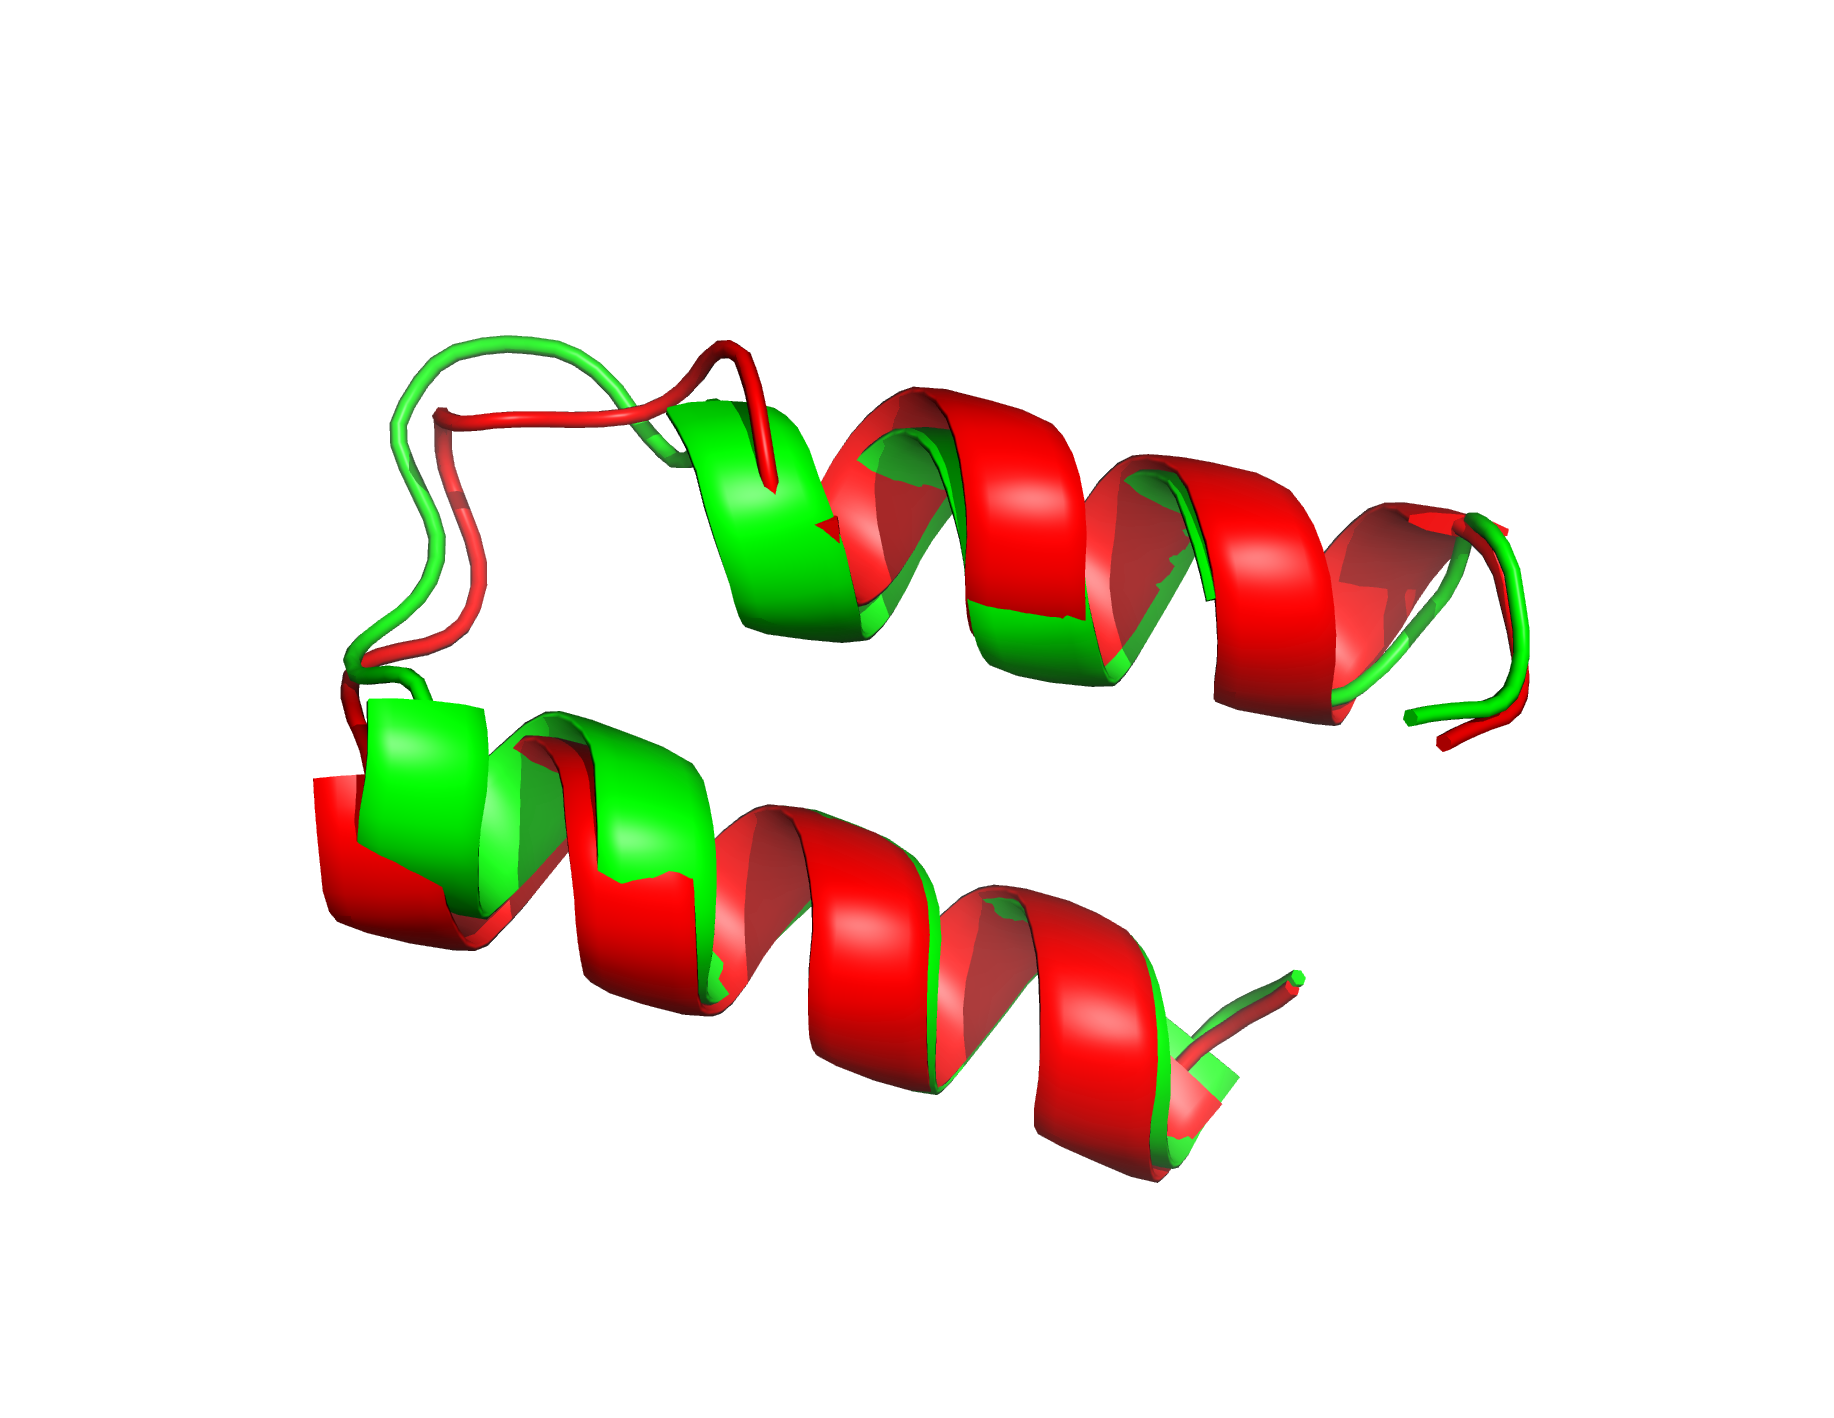
\includegraphics[width=0.9\linewidth]{Figuras/prots/1zdd_render.png}
    \caption{1zdd (1.07\AA)}
    \label{fig:1zdd-conformation}
  \end{subfigure}
%
  \begin{subfigure}{0.32\linewidth}
    \centering
    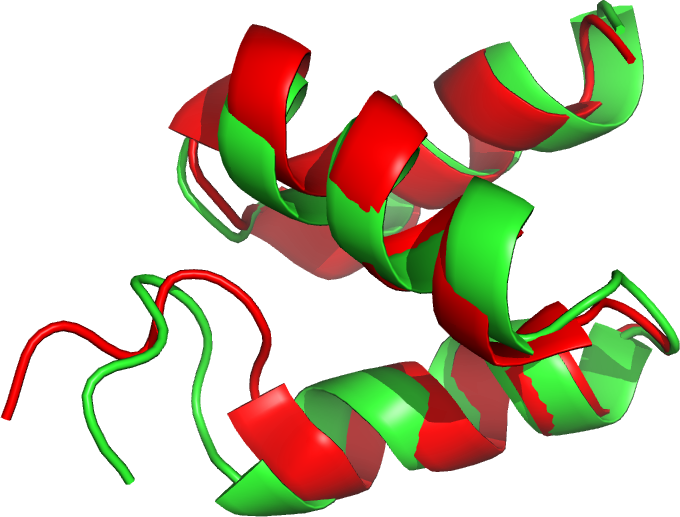
\includegraphics[width=0.9\linewidth]{Figuras/prots/2mr9_render.png}
    \caption{2mr9 (1.66\AA)}
    \label{fig:2mr9-conformation}
  \end{subfigure}
  \caption{The predicted conformations (in green/light gray) compared to the
  native conformation (in red/darker gray). The RMSD between the predicted and
  native conformation is show between parenthesis.}
  \label{fig:all-conformations}
\end{figure}
